%   This document contains diagrams that are included with the PostScript
%   specific \special command. The diagrams are generated by running the
%   program SUN83-C. The 6 gks_74.ps files produced must then be renamed to
%   sun83-c1.ps to sun83-c6.ps.
%
\documentclass[11pt,nolof]{starlink}

% -----------------------------------------------------------------------------
% ? Document identification
\stardoccategory    {Starlink User Note}
\stardocinitials    {SUN}
\stardocsource      {sun\stardocnumber}
\stardocnumber      {83.13}
\stardocauthors     {D L Terrett}
\stardocdate        {8 December 1995}
\stardoctitle       {GKS --- Graphical Kernel System}
\stardocversion     {1.37}
\stardocmanual      {User's Manual}
\stardocabstract {%
The Graphical Kernel System provides a device independent
graphics plotting library.
}
% ? End of document identification
% -----------------------------------------------------------------------------

% ? Document specific \providecommand or \newenvironment commands.
\providecommand{\key}[1]{\fbox{#1}}

% ? End of document specific commands
% -----------------------------------------------------------------------------
%  Title Page.
%  ===========
\begin{document}
\scfrontmatter


\section{Introduction}
This note describes the release on Starlink of the RAL/ICL GKS graphics
package.

GKS has two major advantages over other graphics packages:
\begin{itemize}

\item It is an international standard and real portability of graphics software
is now possible. An illustration of this is that the NCAR
package---an extensive library of scientific graphics utilities produced by the
National Center for Atmospheric Research in the USA---runs on the RAL/ICL GKS
without any modification, despite the fact that it was developed using a
completely independent GKS implementation.

\item No other package provides the ability to write device independent graphics
programs to the extent that GKS does.
Only with GKS can you write a program that will run, and produce good pictures,
on all devices supported by the implementation, including devices not supported
at the time the program was written.
Programs can nonetheless still fully exploit all the facilities offered by the
hardware.
\end{itemize}
The RAL/ICL GKS implementation has several advantages of its own;
it contains features which are not all found in any other single package:
\begin{itemize}
\item Area fill with several fill styles on \emph{all\/} devices.
\item Cell array supported on dot matrix printers.
\item Multiple fonts.
\item Selective clearing of display surface.
\end{itemize}
\section{Documentation}
The RAL/ICL GKS implementation is described in the
\htmladdnormallink{RAL GKS Guide}{http://www.cis.rl.ac.uk/Activities/RAL-GKS/gksguide.html}{}
and the
\htmladdnormallink{RAL GKS Reference Manual}{http://www.cis.rl.ac.uk/Activities/RAL-GKS/gksref.html}{}
(obtainable
from your Starlink site manager or Starlink user support at RAL).
Appendix~\ref{workstations} of this note contains workstation specific
information for devices
for which Starlink has written device handlers.
Where this note and the RAL GKS guide differ this note is correct.

Writers of applications programs may prefer to do low level graphics by means
of the SGS package rather than by using GKS directly.
SGS is described in \xref{SUN/85}{sun85}{} (SGS Users Manual).
Even where a program is pure GKS (perhaps because it has been imported from
another system) you are recommended to take advantage of the workstation name
scheme provided by GNS (\xref{SUN/57}{sun57}{}).

The high level graphics package recommended by Starlink is
\htmladdnormallink{PGPLOT}{http://astro.caltech.edu/~tjp/pgplot/}{}. Programs
that only use PGPLOT for graphics can be linked with either the
``Caltech'' version which is
widely available throughout the world or with a the
\xref{Starlink version}{sun15}{} (SUN/15)
which uses GKS for driving graphics devices. If the Starlink version
is used, other Starlink graphics packages can also be used from the same
program.

\section{Workstation Types}
The workstation types for all the drivers distributed by Starlink are
listed in Tables \ref{terminals}--\ref{metafiles}.
Additional local devices may
have been added; consult your site manager for more information.

The support categories are as follows:
\begin{itemize}
\item S---Supported by Starlink. See Appendix~\ref{workstations} of
this document for more
information.
\item O---Obsolete device, limited support only. See
Appendix~\ref{workstations}.
\item C---Supported by RAL Computing Division; more details can be found in
Appendix~C of the
\htmladdnormallink{RAL GKS
Guide}{http://www.rl.ac.uk/departments/ccd/graphics/ralgks/gksguide.html}{}.
\item U---Not supported; no documentation available.
\item T---\TeX\ specific workstation. See {\xref{SUN/9}{sun9}{}}.
\end{itemize}

\begin{table}\caption{Graphics Terminals}\label{terminals}
\[\begin{tabular}{|l|c|c|c|}\hline
\multicolumn{1}{|c|}{Description} &Workstation type &Support &Page No.\\\hline
Tektronix 4010                      & 201 &C &-\\
Tektronix 4014                      & 203 &C &-\\
Cifer 2634                          & 800 &O &\pageref{cifgt}\\
Cifer T5                            & 801 &O &\pageref{cifgt}\\
Pericom MG/Graphpack                & 820 &O &\pageref{pergt}\\
Pericom MG (RAL mods)               & 821 &O &\pageref{pergt}\\
Pericom 7800                        & 825 &O &\pageref{pergt}\\
GraphOn 235                         & 845 &O &\pageref{gragt}\\
Regis graphics monchrome            &1720 &U &-\\
Regis graphics colour               &1721 &U &-\\
\hline\end{tabular}\]\end{table}

\begin{table}\caption{Laser Printers}
\[\begin{tabular}{|l|c|c|c|}\hline
\multicolumn{1}{|c|}{Description} &Workstation type &Support &Page No.\\\hline
Canon LBP-8 A2/II (landscape)                &2600 &S &\pageref{can}\\
Canon LBP-8 A2/II (portrait)                 &2601 &S &\pageref{can}\\
Canon LBP-8 for \TeX\ (landscape)            &2610 &T &\pageref{can}\\
Canon LBP-8 for \TeX\ (portrait)             &2611 &T &\pageref{can}\\
Postscript (portrait)                        &2700 &C &\pageref{ps}\\
Postscript (landscape)                       &2701 &C &\pageref{ps}\\
EPSF Postscript (portrait)                   &2702 &C &\pageref{ps}\\
EPSF Postscript (landscape)                  &2703 &C &\pageref{ps}\\
Colour Postscript (portrait)                 &2720 &C &\pageref{ps}\\
Colour Postscript (landscape)                &2721 &C &\pageref{ps}\\
Colour EPSF Postscript (portrait)            &2722 &C &\pageref{ps}\\
Colour EPSF Postscript (landscape)           &2723 &C &\pageref{ps}\\
\hline\end{tabular}\]\end{table}

\begin{table}\caption{Workstations}
\[\begin{tabular}{|l|c|c|c|}\hline
\multicolumn{1}{|c|}{Description} &Workstation type &Support &Page No.\\\hline
X-Windows                             &3800 &S &\pageref{xwin}\\
X-Windows                             &3801 &S &\pageref{xwin}\\
X-Windows                             &3802 &S &\pageref{xwin}\\
X-Windows                             &3803 &S &\pageref{xwin}\\
X-Windows overlay                     &3805 &S &\pageref{xwin}\\
X-Windows overlay                     &3806 &S &\pageref{xwin}\\
X-Windows overlay                     &3807 &S &\pageref{xwin}\\
X-Windows overlay                     &3808 &S &\pageref{xwin}\\
\hline\end{tabular}\]\end{table}

\begin{table}\caption{Metafile Workstations}\label{metafiles}
\[\begin{tabular}{|l|c|c|}\hline
\multicolumn{1}{|c|}{Description} &Workstation type &Support\\\hline
Metafile input (Annex E)  &10  &C\\
Computer Graphics Metafile input &12  &C\\
Metafile output (Annex E) &50  &C\\
Computer Graphics Metafile output &52  &C\\
\hline\end{tabular}\]\end{table}

\section{Connection Identifiers}
The connection identifier is used to associate a particular physical device
or file with a GKS workstation. The mechanism used depends on the type of
workstation; for all workstations except the X windows workstation, the
connection identifier is used as the FORTRAN logical unit for output, and
for interactive workstations the next logical unit (connection identifier$+1$)
is used for input. Note that on most UNIX system, logical units 0, 5 and 6
are pre-connected to `standard error', `standard input' and `standard output'
respectively and so 5 should be used to connect a workstation to your
terminal and 0 and 6 not at all.

The device or file name associated with a connection identifier can be
specified by creating an environment variable of the form \texttt{GCON{\em{nn}}},
where \emph{nn} is the connection identifier (with a leading zero if
necessary)
which translates to the device or file name.
For example, to connect a workstation to a file called \texttt{myplot.ps}
on unit 9 you would type:
\begin{terminalv}
% setenv GCON09 myplot.ps
}\end{terminalv}
If not such environment variable exists then the usual default file names
for FORTAN i/o will be used (typically \texttt{fort.{\em{n}}}).

The X windows driver ignores the connection identifier.

\section{Compiling and Linking GKS programs}
Before compiling a program that uses the GKS include file \texttt{GKS\_PAR}
you must first execute the
command:
\begin{terminalv}
% gks_dev
\end{terminalv}

Programs are linked with GKS by:
\begin{terminalv}
% ld objmodule -L/star/lib `gks_link`
\end{terminalv}

\section{GKS Error Handler}
The error handling routine that is used by default reports errors via the
Starlink Error Reporting System (\xref{SUN/104}{sun104}) and the error
channel parameter passed to \texttt{GOPWK} is ignored.

Using the ERR package for error reporting not only makes GKS's error reporting
the same as other Starlink subroutine libraries, but also allows programs
to detect that GKS has reported an error without having to supply their
own error reporting routine. The following example show how this is
done:
\begin{terminalv}
      INTEGER LASTER

*   Include GKS error codes
      INCLUDE 'GKS_ERR'

*   Call GKS routines....
....

*   Call err to see if an error has been reported
      CALL ERR_STAT(LASTER)

*   See if it was a GKS error
      IF ( LASTER .EQ. GKS__ERRROR ) THEN

*      Yes...
...

      ELSE

*      No...
...
      END IF
...
\end{terminalv}

\section{External Names}
All the routines and common blocks visible to the linker, other than the
names specified in the GKS standard, begin with the letters GK.

\section{Fonts}
In addition to the default font (font number 1) the following software fonts
are available on all workstations:

\[\begin{tabular}{|c|l|}\hline
Font number &\multicolumn{1}{|c|}{Description}\\\hline
 -101 &Roman, Medium, Sans serif\\
 -102 &Roman, Bold, Sans serif\\
 -103 &Greek, Medium, Sans serif\\
 -104 &Roman, Medium, Seriffed\\
 -105 &Roman, Italic, Seriffed\\
 -106 &Roman, Bold, Seriffed\\
 -107 &Roman, Bold Italic, Seriffed\\
 -110 &Greek, Medium, Seriffed\\
 -115 &Mathematical\\\hline
\end{tabular}\]
These fonts are illustrated in Appendix~\ref{fonts}.
\section{GKS standards}
GKS is an international standard and yet several ``versions'' exist.
This section is intended to clear up any confusion that may exist.

During the development of the standard, GKS evolved a great deal.
Each revision of the standard document was allocated a number and versions of
the draft standard are referred to by these numbers.
These documents are drafts; there is only one GKS standard; the document finally
adopted by ISO as an international standard.

The first draft that is of more than historical interest is version~6.2, because
this version was implemented by the Technische Hochshule Darmstadt and obtained
at an early date by Starlink.
At that time there was no draft FORTRAN binding (the subroutine names and
argument lists) and the names were invented by Darmstadt.

The RAL/ICL GKS is an implementation of the 7.4 draft
is the version adopted as an ISO standard

\section{Reporting Bugs and Problems}
Problems and suspected bugs should be reported to \texttt{starlink@jiscmail.ac.uk}.
Bugs will be verified and then, if the problem is not in a Starlink written
device driver, reported to Computing Services Division graphics section.

\section{Screen clear suppression}
When a GKS workstation is opened, the display surface is cleared.
For some data reduction system architectures this is inappropriate as it
prevents one applications program from adding to or interacting with a picture
drawn by another.
To circumvent this difficulty, Starlink has implemented an escape function which
suppresses the screen clearing.
This facility should only be used where absolutely necessary as it is unique to
Starlink's GKS and is only available on devices with device handlers written
or modified by Starlink.
It is only available for interactive devices where other techniques such as the
use of metafiles to redraw pictures are too slow to be useful.

To enable the suppression of screen clearing on those devices that support it,
the GKS routine GESC should be called with escape function identifier 1000 and
an ASCII value of 1 as the first character of the data record. The feature is
disabled by 0 in the first character.

An SGS function to access this facility is available and this should be used
wherever possible because the details of the parameters may change in the future
as function identifier values are registered with ISO.

\newpage\appendix
\section{Workstation Specific Information}\label{workstations}

\providecommand{\sect}[1]{\textbf{#1}}

\subsection{Cifer Graphics Terminals}
\label{cifgt}

\sect{Workstation types}

\[\begin{tabular}{|l|l|}\hline
800 &Cifer 2634\\
801 &Cifer T5\\\hline
\end{tabular}\]

\sect{Operation}

\begin{description}
\item[2634]
On open workstation the terminal switches to graphics mode and only the
graphics screen is displayed.
The terminal remains in graphics mode until the workstation is closed when it is
switched back to alpha mode.
\item[T5]
On Open Workstation both the Text and Graphics screens are displayed.
To view the graphics screen only, press \key{SHIFT} + \key{F19}, to view
the alpha screen press \key{SHIFT} + \key{F18}.
To view both, press \key{SHIFT} + \key{F20}.
The screen being viewed can be changed while plotting is in progress.
\end{description}

\sect{Input devices}

\begin{description}
\item[Locator] A cross hair cursor.
Press any key to indicate a point.
The break character is \key{Control}+Z.
\item[Stroke] A cross hair cursor.
Press any key except \key{Return} to indicate a point.
The \key{Return} key signals the end of the entire stroke input.
The break character is \key{Control}+Z.
\item[Valuator] A value typed on the keyboard.
Anything but a valid floating point number is a break.
The prompt and echo will appear on the alpha screen.
\item[Choice] A single digit typed on the keyboard.
Any other key is a break.
The prompt and echo will appear on the alpha screen.
\end{description}

\sect{Deficiencies}

\begin{itemize}
\item String and Pick devices not implemented.
\item Initialization of input devices not implemented.
\end{itemize}

\subsection{Pericom Graphics Terminals}
\label{pergt}

\sect{Workstation types}

\[\begin{tabular}{|l|l|}\hline
820 &Pericom Graphpack/MG series\\
821 &Pericom Graphpack/MG (RAL mods)\\
825 &Pericom 7800\\\hline
\end{tabular}\]

The Graphpack terminals have two blue keys and four white keys at the right hand
side of the keyboard; on a 7800 terminal these keys are grey.
The important difference between the two models is that the Graphpack is capable
of displaying both the alpha and graphics screens simultaneously while the 7800
is not.

\sect{Operation}

\begin{description}
\item[7800] On open workstation the terminal switches to graphics mode and
only the graphics screen is displayed.
The terminal remains in graphics mode until the workstation is closed when it is
switched back to alpha mode; this causes the graphics screen to become
invisible.
The graphics screen can be viewed by pressing the \key{SHIFT}+\key{GRAPH},
and the alpha screen viewed by pressing \key{Control}+\key{GRAPH}.
The terminal must not be switched into alpha mode during plotting.
\item[Graphpack] On Open Workstation both the Text and Graphics screens
are displayed.
To view the graphics screen only press the \key{GRAPH} key, to view
the alpha screen press \key{VDU}.
To view both, press both keys simultaneously and release the key corresponding
to the mode you want the terminal in, second.
The mode of the terminal can be changed while plotting provided that the
terminal is not actually executing graphics commands.

The following terminal setups must be set:
\[\begin{tabular}{lll}
SETUP G &block r &xx01\\
        &block v &0001\\
\end{tabular}\]
The equivalent on an MG series are:
\[\begin{tabular}{ll}
Graphics General   &M) CR Status term\\
Graphics General   &L) ESC=ESC\\
Graphics Modes     &D) Pericom 4014 graphics\\
Graphics Directory &H) GS/CAN Sets Term. Only\\
\end{tabular}\]
\end{description}

\sect{Input devices}

\begin{description}
\item[Locator] A cross hair cursor.
Press any key to indicate a point.
The break character is \key{Control}+Z.
\item[Stroke] A cross hair cursor.
Press any key except \key{Return} to indicate a point.
The \key{Return} key signals the end of the entire stroke input.
The break character is \key{Control}+Z.
\item[Valuator] A value typed on the keyboard.
Anything but a valid floating point number is a break.
The prompt and echo will appear on the alpha screen.
\item[Choice] A single digit typed on the keyboard.
Any other key is a break.
The prompt and echo will appear on the alpha screen.
\end{description}

\sect{Deficiencies}

\begin{itemize}
\item String and Pick devices not implemented.
\item Initialization of input devices not implemented.
\item Hardware dotted lines are not used because of a firmware bug in the
terminal.
\end{itemize}

\subsection{GraphOn 235 Graphics Terminal}
\label{gragt}

\sect{Workstation types}

\[\begin{tabular}{|l|l|}\hline
845 &GraphOn 235\\\hline
\end{tabular}\]

\sect{Operation}

On Open Workstation both the Text and Graphics screens are displayed.

\sect{Input devices}

\begin{description}
\item[Locator] A cross hair cursor.
Press any key to indicate a point.
The break character is \key{Control}+Z.
\item[Stroke] A cross hair cursor.
Press any key except \key{Return} to indicate a point.
The \key{Return} key signals the end of the entire stroke input.
The break character is \key{Control}+Z.
\item[Valuator] A value typed on the keyboard.
Anything but a valid floating point number is a break.
The prompt and echo will appear on the alpha screen.
\item[Choice] A single digit typed on the keyboard.
Any other key is a break.
The prompt and echo will appear on the alpha screen.
\end{description}

\sect{Deficiencies}

\begin{itemize}
\item String and Pick devices not implemented.
\item Initialization of input devices not implemented.
terminal.
\end{itemize}


\subsection{Canon LBP-8 Laser printer}
\label{can}

\sect{Workstation types}

\[\begin{tabular}{|l|l|}\hline
2600 &landscape orientation\\
2601 &portrait orientation\\\hline
\end{tabular}\]

\sect{Operation}
The output from a program that uses these workstations is a file containing a
plot commands.

The file is potentially very large if the Cell Array primitive is used.

\subsection{Postscript}
\label{ps}

\sect{Workstation Types}

\[\begin{tabular}{|l|l|}\hline
2700 &portrait orientation\\
2701 &landscape orientation\\
2702 &EPSF portrait orientation\\
2703 &EPSF landscape orientation\\
2720 &colour portrait orientation\\
2721 &colour landscape orientation\\
2722 &colour EPSF portrait orientation\\
2723 &colour EPSF landscape orientation\\\hline
\end{tabular}\]

\sect{Operation}

The output from a program that uses these workstations is a file containing
postscript commands. The non-EPSF (Encapsulated Postscript Format)
workstations produce a file that is designed printed directly on a Postscript
printer.

The EPSF workstations produce postscript files that can be merged with other
postscript output; for example, inserted into TeX documents - see
\xref{SUN/9}{sun9}{}.

\subsection{X-Windows Server}
\label{xwin}

\sect{Workstation types}

\[\begin{tabular}{|c|c|}\hline
base window &overlay\\\hline
3800 &3805 \\
3801 &3806 \\
3802 &3807 \\
3803 &3808 \\\hline
\end{tabular}\]

\sect{Operation}

When an X workstation is opened the device handler connects to the
default X display (defined by the \texttt{DISPLAY} environment variable)
and searches the display for a GWM
(\xref{Graphics Window Manager}{sun130}{}) window
with the name \texttt{GKS\_{\em{nnnn}}},
where \emph{nnnn} is the workstation type. If the window is
not found it is created. The connection
identifier is ignored and only one workstation of a particular
workstation type can be open at one time.

The size, number of colours and other properties of the window can be
controlled either by using the X resources database or by creating the
window with the \texttt{xmake} command as described in SUN/130. The colours
of colour table entries 0 and 1 are defined by the background and
foreground colours of the window.

Changing the size of the window after the window has been created does
not alter the size of the plotting area.

When the workstation is closed, the window remains on the display and
opening another workstation with the same workstation type will
reconnect to the same window.

An overlay workstation is only available if the window has been created
with an overlay plane (see \xref{SUN/130}{sun130}{xmakeCommand}).

\sect{Input devices}

\begin{description}
\item[Locator] A cross hair cursor.
Press any mouse button except the right hand button to indicate a point. A
break is indicated by pressing the right hand mouse button.
\item[Choice] A single digit typed on the keyboard.
Any other key is a break.
\end{description}

\sect{Deficiencies}

\begin{itemize}
\item Pick device not implemented.
\item String device not implemented.
\item Valuator device not implemented.
\item Hardware text not implemented.
\item Initialization of input devices (except locator position) not implemented.
\item Read pixel and read pixel array not implemented
\end{itemize}

\newpage\section{Font Tables}\label{fonts}

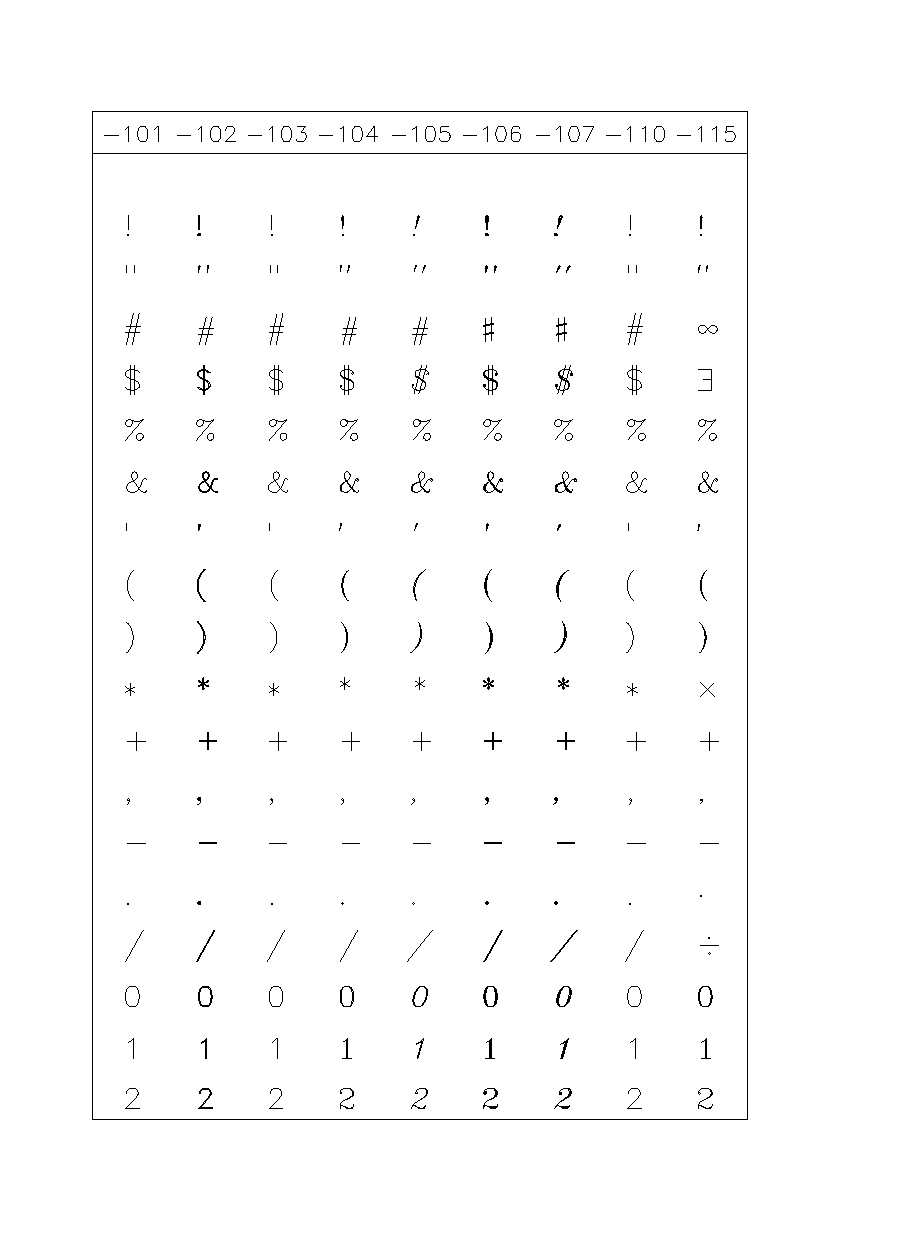
\includegraphics[height=0.95\textheight]{sun83_c1}

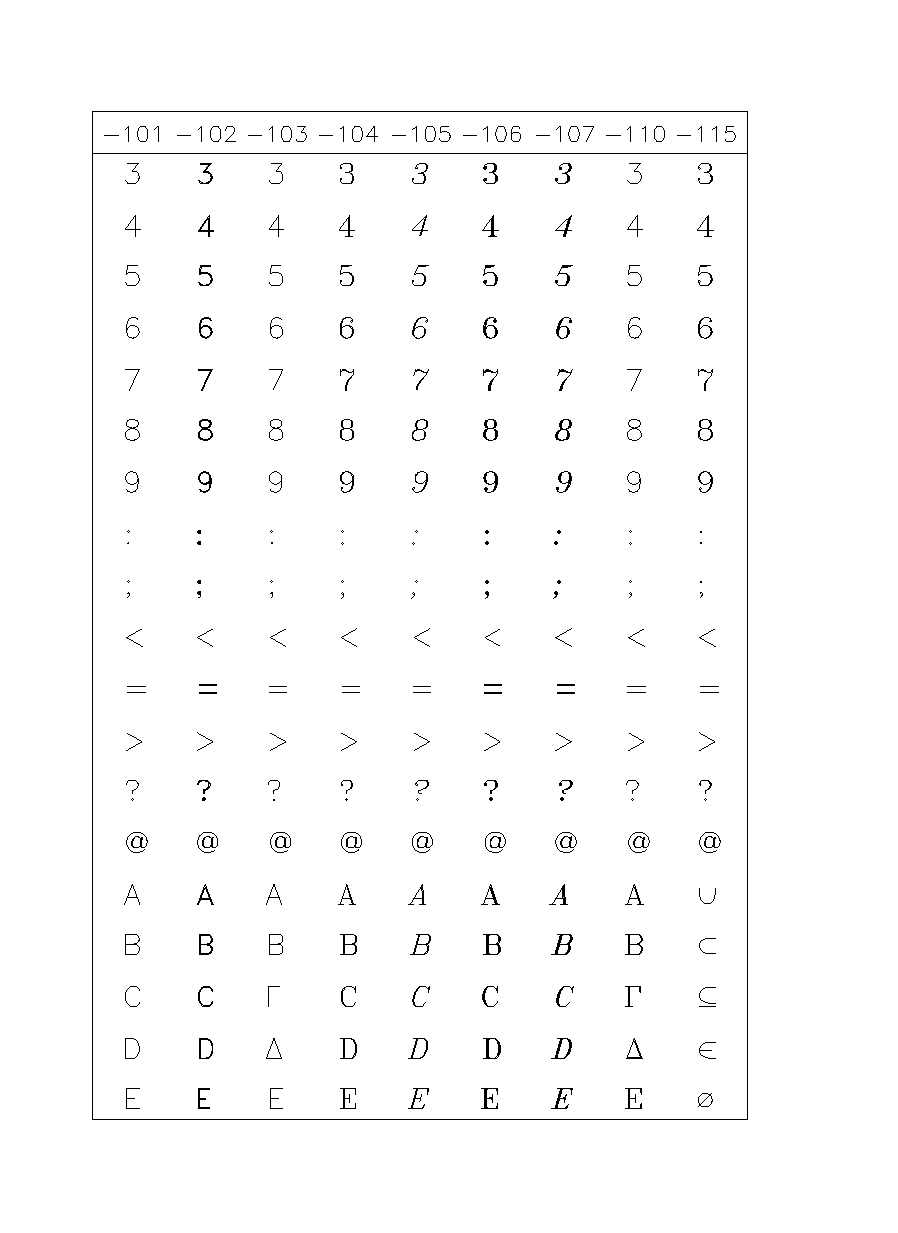
\includegraphics[height=0.95\textheight]{sun83_c2}

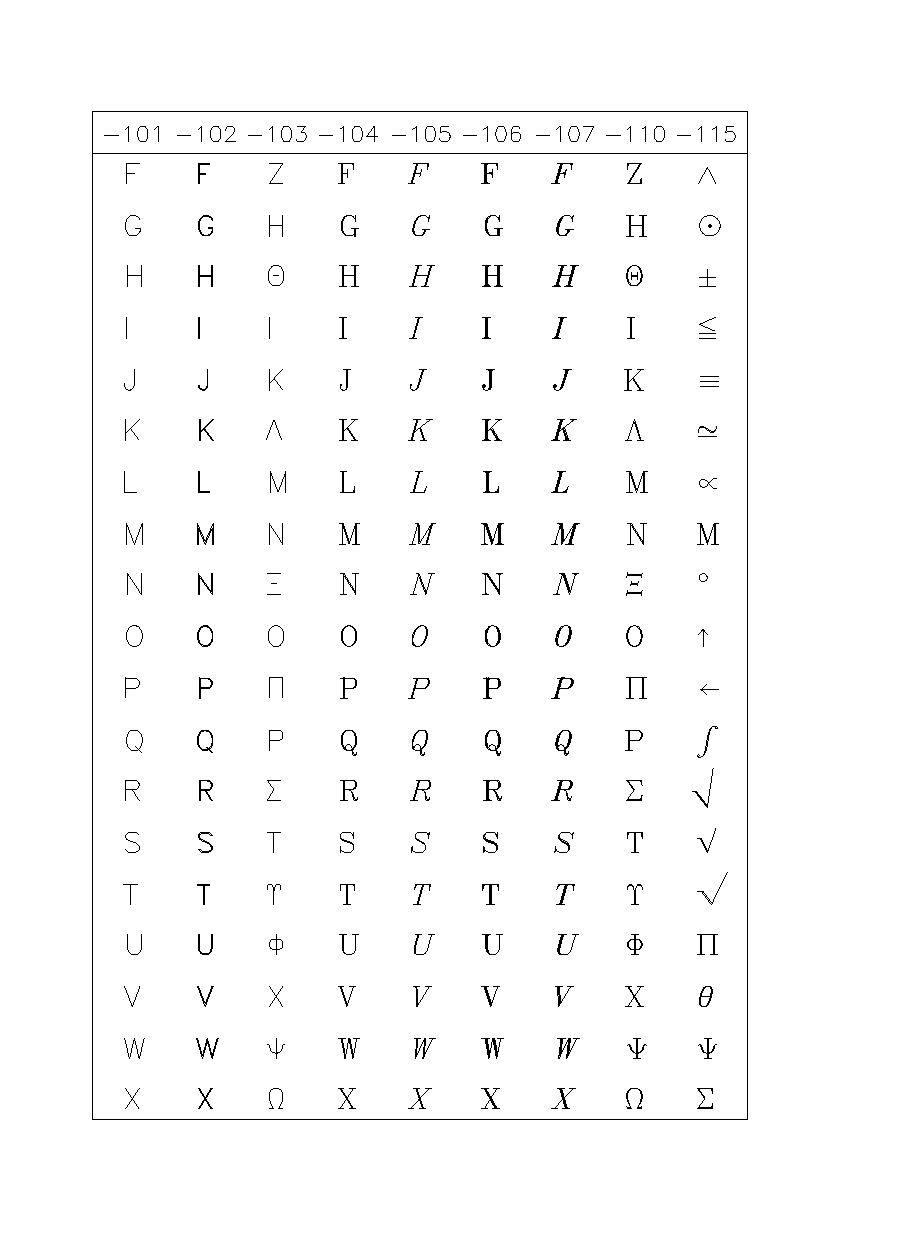
\includegraphics[height=0.95\textheight]{sun83_c3}

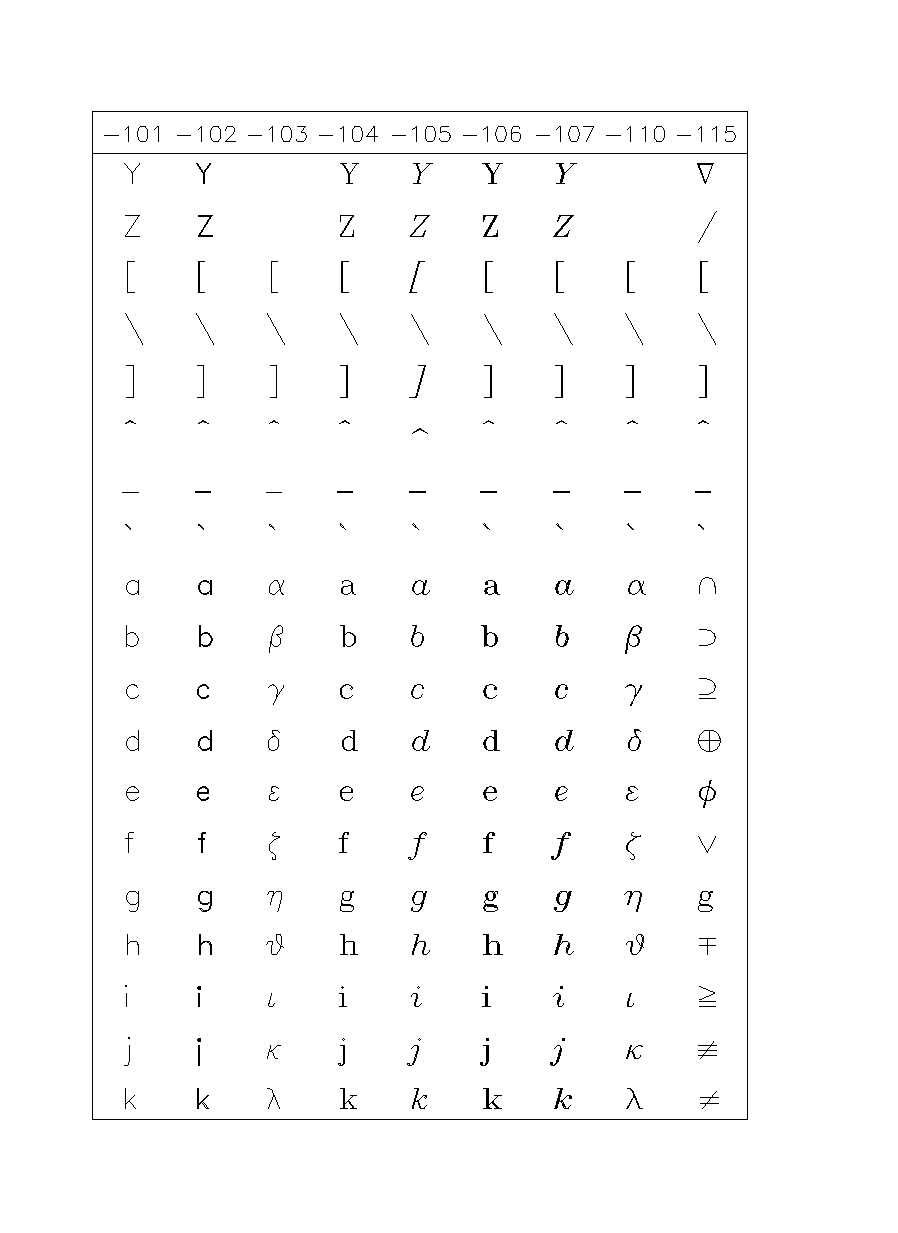
\includegraphics[height=0.95\textheight]{sun83_c4}

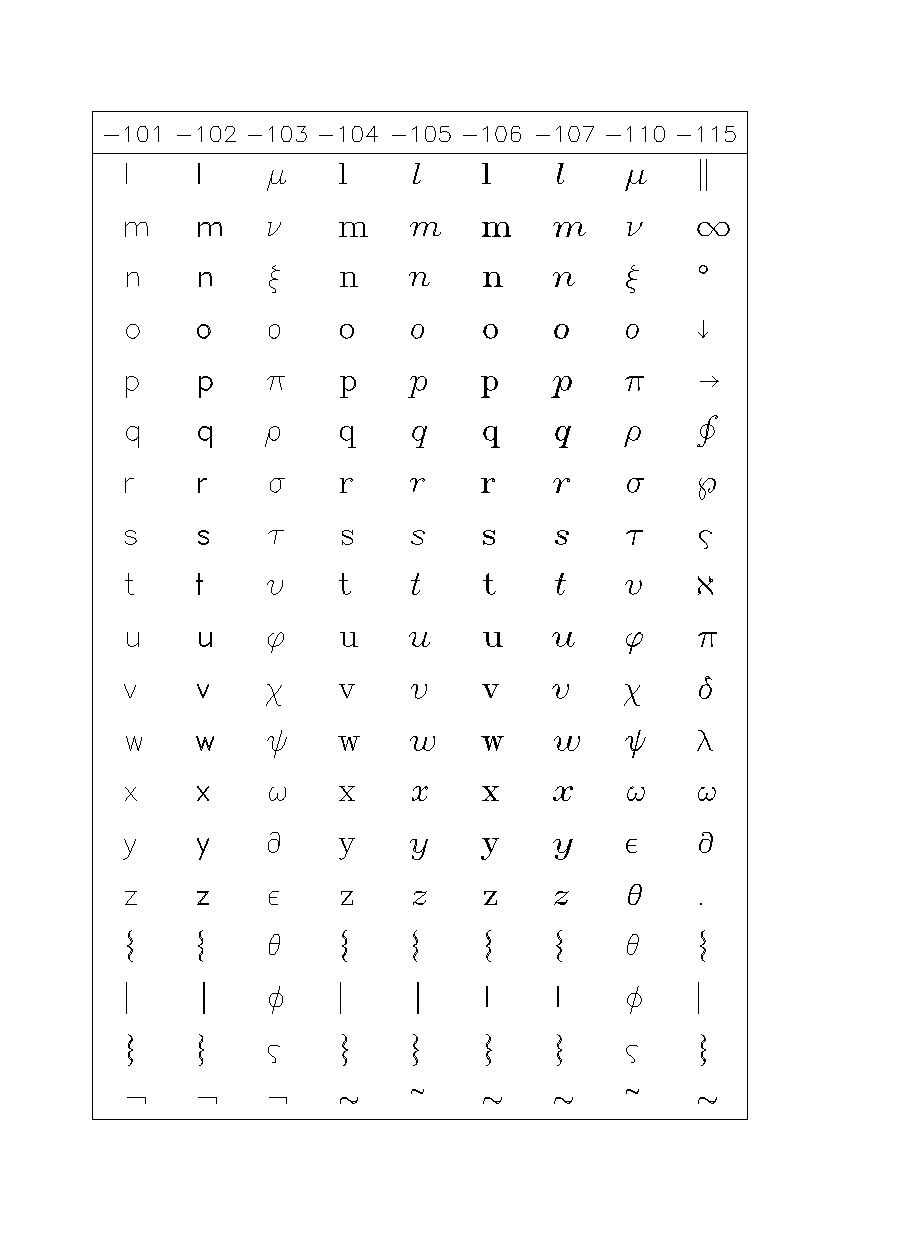
\includegraphics[height=0.95\textheight]{sun83_c5}

\end{document}
